The Reporting Module provides functionality to generate and compare reports
of single/or multiple benchmarks, with the option to export them as csv,
whilst still complying with the quality requirements defined for the system.

\subsection{Architecture Requirements}
\subsubsection{Quality Requirements}
\paragraph*{Flexibility}
The reporting module should be flexible enough to add different elements,
such as graphs, charts and tables. The color scheme should also be easily
changed.

\paragraph*{Performance}
The performance of the reports should as minimalistic as possible, such that the
page is responsive as possible.

\paragraph*{Reliability}
Each report must be reliable with the data it represents, as this is what the
user will be referring to.



\subsection{Architecture Design}
\subsubsection{Architectural Responsibilities, Components and Realization}
The architectural components of the Reporting Module are shown in Figure \ref{fig:reportingResponsibilityAllocation}
\begin{figure}[H]
	\begin{center}
	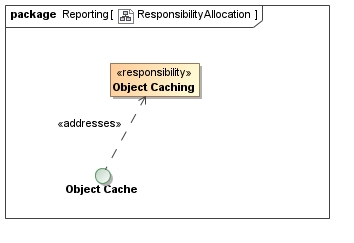
\includegraphics[scale=0.5]{../Diagrams and Charts/Reporting/ResponsibilityAllocation.jpg}
	\caption{The abstract components to which the architectural responsibilities are assigned.}
	\label{fig:reportingResponsibilityAllocation}
	\end{center}
\end{figure}



\subsubsection{Tactics}
The Reporting module should implement the following tactics:
\begin{itemize}
  \item \textit{Report caching} to improve scalability and performance.
\end{itemize}



\subsubsection{Frameworks and Technologies}
The frameworks and technologies used for reporting will consist of JavaScript,
HTML and CSS. With the exporting of reports using a JavaScript library called jsPDF.

We have considered using the jasper reports to generate reports, but it does
 not provide the full functionality that we are looking for. Such as exporting the graphics of the reports.
